\documentclass[aspectratio=169,11pt]{beamer}
\usepackage[T1]{fontenc}
\usepackage{lmodern,amsmath,amssymb,mathtools,bm,booktabs,array,graphicx,tikz}
\usetikzlibrary{arrows.meta,positioning,calc,decorations.pathreplacing,patterns}
\definecolor{ink}{HTML}{17344D}\definecolor{accent}{HTML}{087E8B}\definecolor{pale}{HTML}{EDF5F5}\definecolor{gold}{HTML}{AD6B19}
\providecommand{\dd}{\,\mathrm{d}}\providecommand{\R}{\mathbb{R}}
\providecommand{\E}{\mathbb{E}}\providecommand{\Var}{\operatorname{Var}}
\providecommand{\Cov}{\operatorname{Cov}}\providecommand{\diag}{\operatorname{diag}}
\providecommand{\norm}[1]{\left\lVert#1\right\rVert}
\providecommand{\abs}[1]{\left|#1\right|}
\usefonttheme{professionalfonts}
\setbeamercolor{normal text}{fg=black,bg=white}
\setbeamercolor{frametitle}{fg=ink,bg=white}
\setbeamercolor{title}{fg=ink}\setbeamercolor{structure}{fg=accent}
\setbeamercolor{block title}{fg=ink,bg=pale}\setbeamercolor{block body}{fg=black,bg=pale!40}
\setbeamercolor{alerted text}{fg=accent}
\setbeamerfont{frametitle}{size=\Large,series=\bfseries}
\setbeamerfont{title}{size=\LARGE,series=\bfseries}
\setbeamertemplate{navigation symbols}{}
\setbeamersize{text margin left=.7cm,text margin right=.7cm}
\setbeamertemplate{frametitle}{\vspace{.18cm}\insertframetitle\par\vspace{.1cm}{\color{accent}\hrule height .6pt}\vspace{.12cm}}
\newcommand{\notestarget}{notes.pdf}\newcommand{\noteslabel}{Notes}
\setbeamertemplate{footline}{\hspace{.7cm}\color{ink}\scriptsize Mathematical Modeling\quad\href{\notestarget}{\noteslabel}\hfill\insertframenumber\,/\,\inserttotalframenumber\hspace{.7cm}\vspace{.18cm}}
\setbeamercovered{invisible}
\hypersetup{pdfauthor={Zan Ahmad},pdftitle={Osmotic water transport and cell volume},pdfpagemode=UseNone}
\begin{document}
\begin{frame}[plain]\vfill
{\small\color{accent} Mathematical Modeling \quad Lecture 8}\par\medskip
{\raggedright\hyphenpenalty=10000\exhyphenpenalty=10000\LARGE\bfseries\color{ink} Osmotic water transport and cell volume}\par\bigskip
Zan Ahmad\par\smallskip
{\small Fall 2024}\par\vfill\end{frame}
\renewcommand{\notestarget}{notes.pdf\#note-amount-volume-and-particle-concentration}
\begin{frame}[t,fragile,label=slide-an-impermeant-amount-in-a-changing-volume]{An impermeant amount in a changing volume}
\[n=\text{constant},\qquad c_{\mathrm{in}}=n/V.\]\pause{} Water movement changes concentration without changing trapped solute amount.
\end{frame}
\renewcommand{\notestarget}{notes.pdf\#note-amount-volume-and-particle-concentration}
\begin{frame}[t,fragile,label=slide-concentration-units]{Concentration units}
\[1\,\mathrm{fmol/pL}=\frac{10^{-15}\,\mathrm{mol}}{10^{-12}\,\mathrm L}=1\,\mathrm{mM}.\]\pause{} $300\,\mathrm{fmol}$ in $1\,\mathrm{pL}$ is $300\,\mathrm{mM}$.
\end{frame}
\renewcommand{\notestarget}{notes.pdf\#note-osmotic-pressure-and-a-water-flow-law}
\begin{frame}[t,fragile,label=slide-osmotic-and-hydrostatic-driving-pressures]{Osmotic and hydrostatic driving pressures}
\[\Pi=\mathcal R T c.\]\pause{}\[J_{\mathrm{in}}=L_pA_m\{\Delta\Pi-\Delta P\}.\] Greater internal osmotic pressure draws water inward; greater internal hydrostatic pressure opposes it.
\end{frame}
\renewcommand{\notestarget}{notes.pdf\#note-osmotic-pressure-and-a-water-flow-law}
\begin{frame}[t,fragile,label=slide-conservation-closes-the-scalar-model]{Conservation closes the scalar model}
Equal hydrostatic pressures and constant effective $L$ give\[J_{\mathrm{in}}=L(c_{\mathrm{in}}-c_{\mathrm{out}}).\]\pause{}\[\dot V=L\left(\frac nV-c_{\mathrm{out}}\right).\]
\end{frame}
\renewcommand{\notestarget}{notes.pdf\#note-equilibrium-direction-of-motion-and-stability}
\begin{frame}[label=slide-the-equilibrium-concentration-intersection-figure]{The equilibrium concentration intersection}
\centering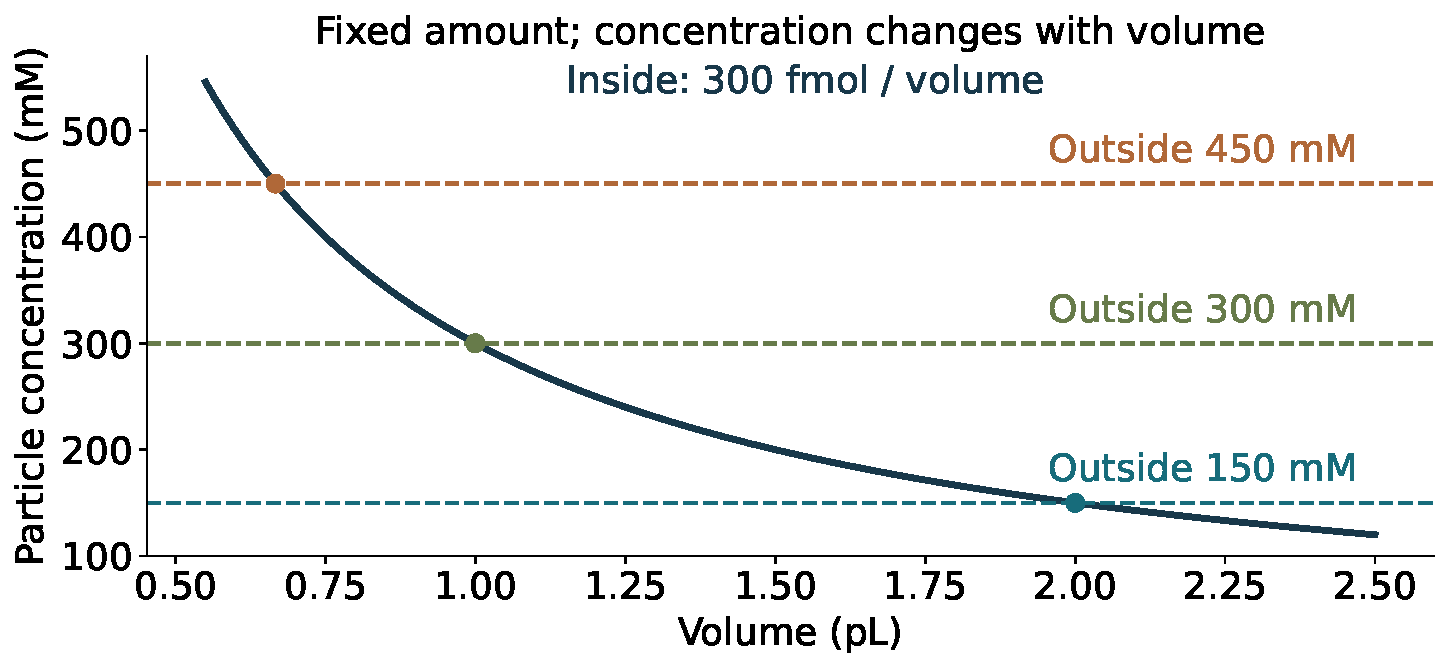
\includegraphics[width=.98\linewidth,height=.69\textheight,keepaspectratio]{osmotic-balance.pdf}\end{frame}
\renewcommand{\notestarget}{notes.pdf\#note-equilibrium-direction-of-motion-and-stability}
\begin{frame}[t,fragile,label=slide-the-equilibrium-concentration-intersection]{The equilibrium concentration intersection}
\[n/V_*=c_{\mathrm{out}}\quad\Longrightarrow\quad V_*=n/c_{\mathrm{out}}.\]\pause{} For $n=300$ and exterior $150,300,450\,\mathrm{mM}$:\[V_*=2,1,2/3\,\mathrm{pL}.\]
\end{frame}
\renewcommand{\notestarget}{notes.pdf\#note-equilibrium-direction-of-motion-and-stability}
\begin{frame}[t,fragile,label=slide-phase-line-analysis]{Phase-line analysis}
\[V<V_*\Rightarrow\dot V>0,\qquad V>V_*\Rightarrow\dot V<0.\]\pause{} The exact solution approaches the equilibrium from its original side.\par\medskip Overshoot in a computed curve may be a time-step artifact.
\end{frame}
\renewcommand{\notestarget}{notes.pdf\#note-equilibrium-direction-of-motion-and-stability}
\begin{frame}[t,fragile,label=slide-local-relaxation-time]{Local relaxation time}
\[V=V_*+\eta:\qquad \dot\eta=-\frac{Ln}{V_*^2}\eta+O(\eta^2).\]\pause{}\[\tau=\frac{V_*^2}{Ln}=\frac n{Lc_{\mathrm{out}}^2}.\]
\end{frame}
\renewcommand{\notestarget}{notes.pdf\#note-dimensionless-dynamics-and-an-implicit-exact-solution}
\begin{frame}[t,fragile,label=slide-a-common-dimensionless-equation]{A common dimensionless equation}
\[v=V/V_*,\qquad\theta=t/\tau.\]\pause{}\[\frac{\dd v}{\dd\theta}=\frac1v-1.\] The reference volume and timescale absorb the constant parameters.
\end{frame}
\renewcommand{\notestarget}{notes.pdf\#note-dimensionless-dynamics-and-an-implicit-exact-solution}
\begin{frame}[t,fragile,label=slide-separation-of-variables]{Separation of variables}
\[\theta=\int_{v_0}^{v}\frac z{1-z}\,\dd z.\]\pause{}\[\theta=v_0-v+\log\left|\frac{1-v_0}{1-v}\right|.\] This formula applies away from the constant equilibrium solution.
\end{frame}
\renewcommand{\notestarget}{notes.pdf\#note-dimensionless-dynamics-and-an-implicit-exact-solution}
\begin{frame}[t,fragile,label=slide-a-decreasing-stability-function]{A decreasing stability function}
\[\Phi(v)=v-1-\log v\geq0.\]\pause{}\[\frac{\dd\Phi}{\dd\theta}=-\left(1-\frac1v\right)^2\leq0.\]
\end{frame}
\renewcommand{\notestarget}{notes.pdf\#note-a-volume-update-and-its-concentration-consequence}
\begin{frame}[t,fragile,label=slide-one-signed-flow-calculation]{One signed flow calculation}
\[J=0.002(300-150)=0.3\,\mathrm{pL/s}.\]\pause{} At $h=0.2\,\mathrm{s}$:\[V^+=1.06\,\mathrm{pL},\qquad c^+=300/1.06\simeq283.019\,\mathrm{mM}.\]
\end{frame}
\renewcommand{\notestarget}{notes.pdf\#note-a-volume-update-and-its-concentration-consequence}
\begin{frame}[t,fragile,label=slide-euler-dynamics-near-equilibrium]{Euler dynamics near equilibrium}
\[\eta_{n+1}\simeq(1-h/\tau)\eta_n.\]\pause{} Stability: $0<h/\tau<2$.\par Nonalternating local relaxation: $0<h/\tau\leq1$.\par\medskip Both differ from an accuracy requirement.
\end{frame}
\renewcommand{\notestarget}{notes.pdf\#note-a-volume-update-and-its-concentration-consequence}
\begin{frame}[label=slide-volume-and-concentration-trajectories-figure]{Volume and concentration trajectories}
\centering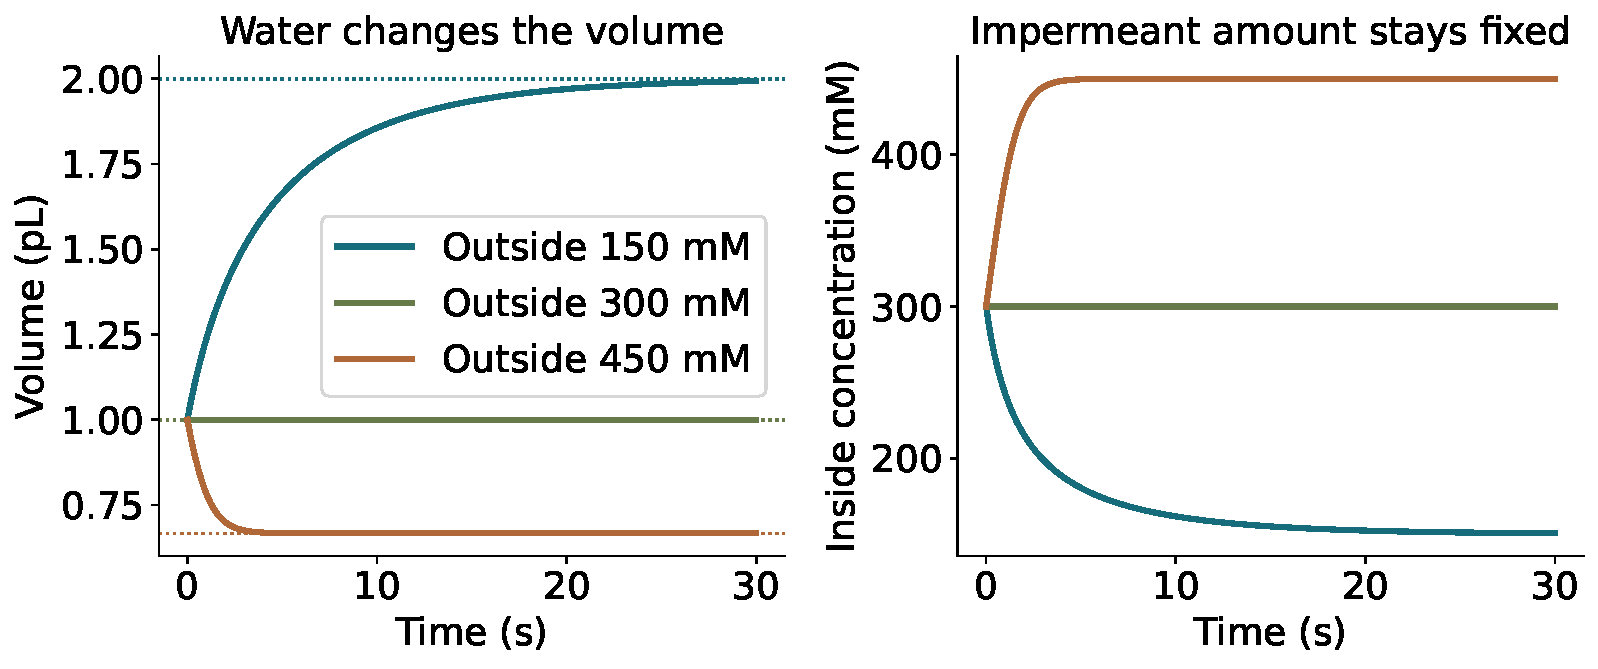
\includegraphics[width=.98\linewidth,height=.69\textheight,keepaspectratio]{volume-trajectories.pdf}\end{frame}
\renewcommand{\notestarget}{notes.pdf\#note-a-volume-update-and-its-concentration-consequence}
\begin{frame}[t,fragile,label=slide-volume-and-concentration-trajectories]{Volume and concentration trajectories}
All cases begin at $V_0=1\,\mathrm{pL}$ with $n=300\,\mathrm{fmol}$.\pause{}\par\medskip Swelling dilutes the trapped solute; shrinking concentrates it.\par\medskip The plotted step is $0.05\,\mathrm{s}$.
\end{frame}
\renewcommand{\notestarget}{notes.pdf\#note-limiting-cases-and-extension-to-volume-regulation}
\begin{frame}[t,fragile,label=slide-zero-external-concentration]{Zero external concentration}
\[\dot V=Ln/V\quad\Longrightarrow\quad\frac{\dd}{\dd t}V^2=2Ln.\]\pause{}\[V(t)=\sqrt{V_0^2+2Lnt}.\] No finite equilibrium exists in this limit.
\end{frame}
\renewcommand{\notestarget}{notes.pdf\#note-limiting-cases-and-extension-to-volume-regulation}
\begin{frame}[t,fragile,label=slide-a-hierarchy-of-numerical-checks]{A hierarchy of numerical checks}
Check $cV=n$, positive volume, and the correct direction of flow.\pause{}\par\medskip Compare against equilibrium, the zero-exterior exact solution, or the implicit trajectory relation.\par\medskip Refine time steps at common times.
\end{frame}
\renewcommand{\notestarget}{notes.pdf\#note-limiting-cases-and-extension-to-volume-regulation}
\begin{frame}[t,fragile,label=slide-additional-mechanisms-for-cell-volume-regulation]{Additional mechanisms for cell-volume regulation}
Permeant ions require amount balances.\par Hydrostatic pressure requires mechanics.\par Active transport requires pump fluxes.\pause{}\par\medskip The present water-only calculation isolates osmosis; it does not establish cell survival or physiological regulation.
\end{frame}
\end{document}
